\documentclass[a4paper,11pt,titlepage]{book}
%\usepackage[utf8]{inputenc}
\usepackage[english]{babel} %if you want the english version
\usepackage{csquotes}
\usepackage[export]{adjustbox}
\usepackage{booktabs}
\usepackage{subfigure}
\usepackage{geometry}
\geometry{a4paper,top=3cm,bottom=3cm,left=3.5cm,right=3.5cm,heightrounded,bindingoffset=3mm}
\usepackage{multicol}
\usepackage{graphicx,xcolor}
\usepackage{fancyhdr}
\renewcommand{\headrulewidth}{0pt}
\usepackage{lipsum}
\usepackage{physics}
\usepackage{amsmath}
\usepackage{amssymb}
\usepackage{amsthm}
\usepackage{leftindex}
\usepackage{anyfontsize}
\usepackage{multirow}
\usepackage{xfrac}
\usepackage{gensymb}
\usepackage{parskip} %to remove paragraph initial indentation
\usepackage[font=small,labelfont=bf]{caption}

%\pagestyle{fancy}

\usepackage[raggedright]{titlesec}
\titleformat*{\subsection}{\large\bfseries}
\titleclass{\chapter}{straight}
%\usepackage{mathptmx}   % Times + simboli matematici
%\usepackage{newtxtext,newtxmath} %this triggers times new roman
%\usepackage{fontspec}

%\setlength{\columnsep}{4cm} %adjust base on your name length

\theoremstyle{plain}
\newtheorem{thm}{Theorem}[chapter] % reset theorem numbering for each chapter

\theoremstyle{definition}
\newtheorem{defn}[thm]{Definition} % definition numbers are dependent on theorem numbers
\newtheorem{ex}[thm]{Example} % same for example numbers

\definecolor{bluep}{RGB}{13, 80, 160}%color of bachelor in physics
\definecolor{redp}{RGB}{229, 7, 47}%unito color
\definecolor{redf}{RGB}{128, 8, 0}%color of master in physics
\definecolor{greenf}{RGB}{75, 118, 64}%color of master in complex systems
\newcommand{\bfcolor}[2]{\textcolor{#1}{\textbf{#2}}}
\newcommand{\fsize}[2]{\fontsize{#1}{#2}\selectfont}
\newcommand{\COMMENT}[1]{} %comment block

%\fancyfoot{}
%\fancyfoot[C]{\thepage}

%\setlength{\headheight}{21pt}

\newenvironment{abstract}{}{}
\usepackage{abstract}

%\usepackage[citecolor=gray]{hyperref}
\usepackage{hyperref}
\usepackage{subcaption} %per fare subfigure
\usepackage{float}
\usepackage{array} %per le table
\usepackage{tabularx}
\hypersetup{
    colorlinks=true,
    linkcolor=black,
    filecolor=red,
    %citecolor=redp,
    citecolor=gray,
    urlcolor=bluep,
}

\usepackage{datetime}
\edef\today{\number\day\
\ifcase\month\or
%Gennaio\or Febbraio\or Marzo\or Aprile\or Maggio\or Giugno\or Luglio\or
%Agosto\or Settembre\or Ottobre\or Novembre\or Dicembre\fi\ \number\year
January\or February\or March\or April\or May\or June\or July\or
August\or September\or October\or November\or December\fi\ \number\year
}


%\usepackage{textblock}
\usepackage[absolute]{textpos}

\renewcommand{\chaptermark}[1]{\markboth{\thechapter.\ #1}{}}
\renewcommand{\sectionmark}[1]{\markright{\thesection.\ #1}}

\fancypagestyle{body}{
    \pagenumbering{arabic}
    \fancyhead[LE,RO]{
    }
    \fancyhead[C]{}
    \fancyhead[LE,RO]{\thepage}
    \fancyhead[RE]{
	\leftmark
    }
    \fancyhead[LO]{
	%\small{\textbf{Università degli studi di Torino}}
    }
    \fancyfoot[C]{}
    \renewcommand{\headrulewidth}{0.4pt}
}
\fancypagestyle{intro}{
    \pagenumbering{roman}
    \fancyhead[L]{
	%TESTINTRO
    }
    \fancyhead[C]{}
    \fancyhead[R]{}
    \fancyfoot[C]{\small{\thepage}}
    \renewcommand{\headrulewidth}{0.0pt}
}

\fancypagestyle{empty}{
    \fancyhead[C]{
	%TESTEMPTY
    }
    \fancyhead[R]{
	%TESTEMPTY
    }
    \fancyhead[L]{
	%TESTEMPTY
    }
    \fancyfoot[C]{
	%TESTEMPTY
    }
    \renewcommand{\headrulewidth}{0.0pt}
}

\usepackage[backend=biber, style=nature, sorting=none, doi=true, url=true]{biblatex}
%\setlength{\bibitemsep}{0.3cm}
\addbibresource{citations.bib}
%\addbibresource{main.bib}


\begin{document}
\pagestyle{empty}
\begingroup


%\begin{figure}
%    \centering
%    \includegraphics[width=4cm]{figures/LogoUniToConvertito.png}
%\end{figure}
\begin{textblock*}{4cm}(8.65cm,2.5cm)
    \centerline{
\includegraphics[width=4.67cm]{./LogoUniToConvertito.png}}
\end{textblock*}
 %textbf per copertina su TUTTO, segnato con %%%

\begin{textblock*}{21cm}(0cm,10cm)
	\fontsize{22}{22}\selectfont
	\centerline{\textbf{Università degli Studi di Torino}}%%%
\end{textblock*}
\begin{textblock*}{21cm}(0cm,11cm)
	\fontsize{18}{22}\selectfont
	\centerline {\textit{Corso di Laurea in Fisica}}
\end{textblock*}


\begin{textblock*}{21cm}(0cm,13.4cm)
	\centering
    \fontsize{28}{24}\selectfont
    \textbf{Metodi Supersimmetrici\\per la Meccanica Quantistica}
\end{textblock*}
\begin{textblock*}{21cm}(0cm,15.6cm)
	\fontsize{19}{22}\selectfont
	\centerline{Tesi di Laurea}%%%
\end{textblock*}



\fontsize{18}{17}\selectfont
\begin{textblock*}{8cm}(3.04cm,18.6cm)
	\noindent 
	\textbf{Relatrice}
\end{textblock*}
%\fontsize{18}{17}\selectfont
\begin{textblock*}{8cm}(3.04cm,19.2cm)
	\noindent 
	Frau Marialuisa%%%
\end{textblock*}




\begin{textblock*}{8cm}(12.33cm,22.95cm)
	\noindent
	\textbf{Candidato}
\end{textblock*}
\begin{textblock*}{8cm}(12.33cm,23.55cm)
	\noindent	\textbf{Rocchietti March Paolo}%%%
\end{textblock*}
\begin{textblock*}{8cm}(12.33cm,24.14cm)
	\noindent	Matricola 1093935
\end{textblock*}


\fontsize{16}{17}\selectfont
\begin{textblock*}{21cm}(0cm,27.34cm)
	\centerline{Anno Accademico 2025/2026}%%%
\end{textblock*}

\endgroup


\null

\newpage
\phantom{easter egg :)}
\newpage
\pagestyle{intro}
\begin{abstract}%sottintende newpage
    \thispagestyle{intro}
In this thesis the formalism of Supersymmetry is applied to non-relativistic
Quantum Mechanics and it is shown how new solvable potentials can be
constructed from known ones. This formalism is then enriched with the concept
of shape invariance, that leads to an algebraic ladder operator method 
for the solutions of certain potentials. Finally a Supersymmetry-inspired
approach to the semi-classical WKB approximation is presented and its advantages
with shape invariant potentials are stated. Some examples for each concept are
provided.

\end{abstract}%sottintende newpage
\thispagestyle{empty}
\phantom{vuota}
\newpage
\thispagestyle{empty}
\tableofcontents
\newpage
\thispagestyle{empty}
\phantom{vuota}
\newpage
\pagestyle{body}
\thispagestyle{empty}
\chapter*{Introduction}
\addcontentsline{toc}{chapter}{Introduction}
The theoretical framework of Supersymmetry is based on the existence of a 
new kind of symmetry in which to each bosonic particle
corresponds a new fermion and to each fermionic particle corresponds a new boson:
these are called superpartner particles and their spin differs from their
"regular" partner's by a half integer. More precisely, Supersymmetry was
introduced in the context of Quantum Field Theories as an internal symmetry
of a Lagrangian between fermionic and bosonic degrees of freedom, as a way to
unify interactions (bosons) with matter (fermions).\\
So far in nature none of these superpartners have been observed and so
it is conjectured that Supersymmetry must be spontaneously broken and
the scale of this breaking is at least of the order of $100$ GeV.

From this context, researchers started to test supersymmetric theories in
simpler theoretical frameworks, like that of non-relativistic Quantum
Mechanics, finding insight on solvable potentials.

In the first chapter of this thesis the formalism and algebraic structure of
Supersymmetric Quantum Mechanics is introduced and the properties of
supersymmetric partner Hamiltonians are stated and proven; some examples
are then provided and explicitely explored. The main references for this
chapter are \cite{cooper_main} and \cite{khare_short} for the definitions and
properties of Supersymmetry and \cite{bastianelli} for the Supersymmetric
Algebra.

In the second chapter of this thesis the concept of shape invariant partner
potentials is introduced with their properties: this definition is then used
to construct a generalization of the ladder operators for the Quantum Harmonic
Oscillator to a greater set of integrable 1-dimensional potentials; finally, some
examples of potentials with complex analytical solutions are solved with the
properties of shape invariance. The main reference for this chapter is again
\cite{cooper_main}. 

In the third and final chapter of this thesis a variation
of the WKB quantization condition on bound states of supersymmetric 
partner potentials is derived for both broken and unbroken supersymmetry; it is
then shown that this method yields the exact energy eigenvalues of the spectrum
of shape invariant potentials. The references for this chapter are \cite{zwiebach}
for the general theory on the WKB method and \cite{cooper_main}, \cite{dutt_swkb}
for the supersymmetric approach.

\newpage
%------------------------------------------------------------------------------------------------
\chapter{Supersymmetric Quantum Mechanics}
\thispagestyle{empty}
Here the formalism of Hamiltonian 1-dimensional supersymmetric Quantum Mechanics 
is introduced, then its fundamental properties will be stated and proven; in the
end, some applications to 1-dimensional and 3-dimensional potentials will be
explored in detail.
\section{First definitions}
The fundamental structure of supersymmetric Quantum Mechanics is based on two
operators:
\begin{gather*}
\hat A = \frac{\hbar}{\sqrt{2m}}\dv[]{}{x} + W(x)\\
\hat A^\dagger = -\frac{\hbar}{\sqrt{2m}}\dv[]{}{x} + W(x).
\end{gather*}
that will be used to construct two Hamiltonians.
\begin{defn}
The real function $W(x)$ is called \textit{superpotential}.
\end{defn}
\begin{defn}
The self-adjoint operators
\begin{gather}
\hat H_1 := \hat A^\dagger\hat A \label{def:H1}\\
\hat H_2 := \hat A\hat A^\dagger \label{def:H2}
\end{gather}
are called \textit{supersymmetric partners Hamiltonians}, and it is trivial to show that
\begin{gather*}
\hat H_1 = -\frac{\hbar^2}{2m}\dv[2]{}{x} + V_1(x)\\
\hat H_2 = -\frac{\hbar^2}{2m}\dv[2]{}{x} + V_2(x),
\end{gather*}
where 
\begin{gather}
V_1(x) = W^2(x)-\frac{\hbar}{\sqrt{2m}}W'(x)\label{eq:V_1}\\
V_2(x) = W^2(x)+\frac{\hbar}{\sqrt{2m}}W'(x)\label{eq:V_2}.
\end{gather}
\end{defn}
These definitions employ the typical language of supersymmetric theories: its
fundamental algebraic structure will now be briefly introduced.
\newpage
\section{Hints at supersymmetric Algebra}
\label{sec:susy_algebra}
Similarly to classical Hamiltonian mechanics, in Quantum Mechanics every symmetry
is closely related to an operator commuting with the
Hamiltonian of the system: Supersymmetry can also be defined in similar terms.

Given the operators defined earlier, consider the operators

\begin{equation*}
\hat Q = \begin{pmatrix}
    \mathbb{O}&\mathbb{O}\\
    \hat A&\mathbb{O}
\end{pmatrix}\text{,   }
\hat Q^\dagger = \begin{pmatrix}
    \mathbb{O}&\hat A^\dagger\\
    \mathbb{O}&\mathbb{O}
\end{pmatrix}
\label{eq:alg_1}
\end{equation*}
and the Hamiltonian
\begin{equation*}
\hat H := \left\{\hat Q,\hat Q^\dagger\right\}= 
\begin{pmatrix}
    \hat A^\dagger\hat A& \mathbb{O}\\
    \mathbb{O}&\hat A\hat A^\dagger
\end{pmatrix} =
\begin{pmatrix}
    \hat H_1& \mathbb{O}\\
    \mathbb{O}&\hat H_2
\end{pmatrix},
\end{equation*}

The (vector) ground state of $\hat H$ is
$$\psi_0=\begin{pmatrix}
\psi^{(1)}_0\\
\psi^{(2)}_0
\end{pmatrix},
$$
where $\psi^{(i)}_0$ are the ground states of $\hat H_i$.

The definition of the Hamiltonian $\hat H$ is the first property of the
supersymmetric Algebra, the others follow from the definitions of $\hat Q$ and
$\hat H$:
\begin{equation*}
\left[\hat H, \hat Q\right]= \left[\hat H, \hat Q^\dagger\right]=0
\end{equation*}
and 
\begin{equation*}
\left\{\hat Q,\hat Q\right\}=\left\{\hat Q^\dagger,\hat Q^\dagger\right\}=0.
\label{eq:alg_2}
\end{equation*}
\textbf{Note} The symmetry is given by the fact that $\hat Q,\; \hat Q^\dagger$
commute with the Hamiltonian of the system.

To introduce the concept of supersymmetry breaking, some properties of the
partner Hamiltonians need to be considered.

%\begin{defn}
%The conditions (\ref{eq:alg_1}) to (\ref{eq:alg_2}) define a Lie Superalgebra.
%\end{defn}%forse inutile

\COMMENT{
\begin{defn}
Supersymmetry is \textbf{spontaneously broken} if and only if
\begin{equation*}
\hat Q \psi_0 \neq0,\quad\hat Q^\dagger\psi_0\neq0.
\end{equation*}
\label{def:b_algebra}
\end{defn}
\begin{defn}
Supersymmetry is \textbf{unbroken}
if and only if
\begin{equation*}
\hat Q \psi_0 = \hat Q^\dagger\psi_0=0.
\end{equation*}\label{def:unb_algebra}
\end{defn}
These definitions are inspired by the definition of broken symmetries in Quantum
Mechanics.
\newpage}
\section{Fundamental properties of supersymmetric partners}
The most interesting properties of supersymmetric partner Hamiltonians lie in the
relationships between their energy spectra and corresponding eigenstates.

\begin{thm}
Supersymmetric partner Hamiltonians admit only non-negative eigenvalues.
\end{thm}
\textbf{Proof} Consider the Hamiltonians $\hat H_1, \hat H_2$: $\forall\ket{\psi}$ the
quantities
\begin{gather*}
\bra{\psi}\hat H_1\ket{\psi} = \bra{\psi}(\hat A^\dagger\hat A)\ket{\psi} = 
\left|\left| \hat A \ket{\psi} \right|\right|^2\\
\bra{\psi}\hat H_2\ket{\psi} = \bra{\psi}(\hat A\hat A^\dagger)\ket{\psi} = 
\left|\left| \hat A^\dagger \ket{\psi} \right|\right|^2
\end{gather*}
are non-negative, thus proving the statement.\qed\\

In addition to this interesting property, supersymmetric partner Hamiltonians' spectra are
related, due to the fact that they are constructed with the same two operators:
consider the eigenstate $\ket{E^{(1)}}$ for $\hat H_1$ with eigenvalue $E$,
such that
$$\hat H_1 \ket{E^{(1)}} = E \ket{E^{(1)}}.$$
Applying the operator $\hat A$ to both sides yields
$$\hat A\hat H_1\ket{E^{(1)}} = E\hat A\ket{E^{(1)}}.$$
Recalling (\ref{def:H1}) and (\ref{def:H2}),
\textbf{if} $\mathbf{\hat A\ket{E^{(1)}}\neq0}$ (thus $E\neq0$), this is
equivalent to
$$\hat A\hat A^\dagger\hat A\ket{E^{(1)}} = E \hat A \ket{E^{(1)}}
\Rightarrow \hat H_2\hat A \ket{E^{(1)}} =
E\hat A\ket{E^{(1)}}.$$
This shows that the state
\begin{equation}
    \ket{{E^{(2)}}} :=\frac{1}{\sqrt{E}}\hat A\ket{E^{(1)}}
\label{eq:A_use}
\end{equation}
is a normalized eigenstate of $\hat H_2$ with eigenvalue $E$.

Similarly, it can be shown that for an eigenstate $\ket{E^{(2)}}$ of $\hat H_2$,
\textbf{if} $\mathbf{\hat A^\dagger\ket{E^{(2)}}\neq0}$, the state
\begin{equation}
\ket{E^{(1)}} :=\frac{1}{\sqrt{E}}\hat A^\dagger\ket{E^{(2)}}
\label{eq:A+_use}
\end{equation}
is a normalized eigenstate of $\hat H_1$ with eigenvalue $E$.

If, on the other hand, $\hat A \ket{E^{(1)}}=0$ or
$\hat A^\dagger \ket{E^{(2)}}=0$, the eigenvalue of both these eigenstates
must be $E=0$; to see the implications of this condition, it is useful to consider
the energy spectra of $\hat H_1,\hat H_2$ to be discrete, and so from this point
onwards the eigenfunctions and eigenvalues of the Hamiltonians will be denoted as
$$\hat H_i \psi^{(i)}_n = E^{(i)}_n\psi^{(i)}_n.$$
Consider now the case $\hat A \psi_n^{(1)}=0$: this implies $\hat H_1 \psi^{(1)}_n=0$, i.e. that
the wavefunction annihilated by $\hat A$ is the ground state of $\hat H_1$, with eigenvalue
$E^{(1)}_0=0$; this equality yields an analytic expression for the ground state of $\hat H_1$:
\begin{gather*}
\hat A \psi^{(1)}_0 = 0 \iff \frac{\hbar}{\sqrt{2m}}\dv[]{}{x}\psi^{(1)}_0(x) =
W(x)\psi^{(1)}_0 \iff \frac{\dd \psi^{(1)}_0}{\psi^{(1)}_0}=
-\frac{\sqrt{2m}}{\hbar}W(x)
\end{gather*}
\begin{equation}
\psi^{(1)}_0(x)=N\exp\left[-\frac{\sqrt{2m}}{\hbar}\int_{x_0}^{x}\dd y W(y)\right].
\label{eq:ground_state}
\end{equation}
\textbf{Note} For this to be a true ground state wavefunction, it must be
continuous and normalizable: this is true if the integral function
$$f(x) = \int_{x_0}^x \dd y W(y)$$
is continuous and if
$$\lim\limits_{x\to\pm\infty}\frac{f(x)}{\ln(\pm x)}=+\infty:$$
this means that $f$ must increase at $+\infty$ and decrease at $-\infty$, since
$f(x)$ is the integral function of $W(x)$, this implies that
\begin{equation}
\begin{dcases}
      0\leq\lim\limits_{x\to+\infty} W(x) \leq+\infty\\
      -\infty\leq\lim\limits_{x\to-\infty}W(x)\leq 0.
  \end{dcases}
    \label{eq:lim_W}
\end{equation}


If the ground state is known, $\hat A \psi^{(1)}_0=0$ provides an expression for
the superpotential
\begin{equation}
W(x)=-\frac{\hbar}{\sqrt{2m}}\frac{\psi'^{(1)}_0(x)}{\psi^{(1)}_0(x)}.
\label{eq:W_ground}
\end{equation}
These considerations about the ground state can be similarly derived using $\hat H_2$, from
$\hat A^\dagger \psi^{(2)}_0=0$:
\begin{gather*}
\psi^{(2)}_0(x)=N\exp\left[\frac{\sqrt{2m}}{\hbar}\int_{x_0}^{x}\dd y W(y)\right],\\
\lim\limits_{x\to\pm\infty}\frac{f(x)}{\ln(\pm x)}=-\infty\implies\begin{dcases*}
-\infty\leq\lim\limits_{x\to+\infty}W(x)\leq0\\
0\leq\lim\limits_{x\to-\infty}W(x)\leq+\infty
\end{dcases*},\\
W(x)=\frac{\hbar}{\sqrt{2m}}\frac{\psi'^{(2)}_0(x)}{\psi^{(2)}_0(x)}.
\end{gather*}
It is easy to show that these two conditions (and so two $E=0$ ground states) cannot cohexist:
\begin{thm}
Only one of the two ground states of partner Hamiltonians can have eigenvalue $E^{(i)}_0=0$.
\end{thm}

\textbf{Proof (by contradiction)} Suppose both ground states have
$E^{(1)}_0 = E^{(2)}_0=0$: by the previous calculations, their wavefunctions are

$$\begin{aligned}
&\psi^{(1)}_0 = N\exp\left[-f(x)\right]\\
&\psi^{(2)}_0 = N\exp\left[f(x)\right]
\end{aligned}\text{  with } f(x)=\frac{\sqrt{2m}}{\hbar}\int_{x_0}^{x}\dd y W(y)
$$
it is clear that these two wavefunctions cannot be simultaneously normalized, a contradiction.
\qed\\

\textbf{Note} From this point, the superpotential $W(x)$ is chosen so that only the
Hamiltonian $\hat H_1$ can possess a $E=0$ ground state.
\newpage
\begin{defn}
Supersymmetry is \textbf{spontaneously broken} if and only if
\label{def:broken_susy}
\end{defn}
$$\hat A \psi^{(1)}_0 \neq0.$$
\begin{defn}
Supersymmetry is \textbf{unbroken} if and only if
\label{def:unbroken_susy}
\end{defn}
$$\hat A \psi^{(1)}_0=0.$$
\textbf{Note}
Since $\hat A\psi^{(1)}_0=0$ is a necessary condition for
(\ref{eq:lim_W}), if the limits of $W(x)$ do not respect these conditions,
Supersymmetry must be spontaneously broken.\\
If Supersymmetry is spontaneously broken, the limits of $W(x)$ can
have any sign save those described in (\ref{eq:lim_W}) and their counterpart
implied by $\hat A \psi^{(2)}_0=0$: this implies that they must have the same
sign.

Another way to define Supersymmetry breaking is through the operators
$\hat Q,\hat Q^\dagger$ defined in Section \ref{sec:susy_algebra}:
$$\hat Q^\dagger \psi_0 = 0 \iff \psi_0^{(2)}\equiv0 \land
\hat A \psi_0^{(1)} =0\iff
\hat Q \psi_0  =0,
$$
so Supersymmetry is unbroken if and only if 
$$\hat Q \psi_0 =\hat Q^\dagger\psi_0=0$$
which closely resembles the definition of spontaneous symmetry breaking in Quantum
Mechanics.

For both broken and unbroken Supersymmetry, the peculiar property of supersymmetric
partner Hamiltonians is expressed in equations (\ref{eq:A_use}) and (\ref{eq:A+_use}):
for discrete spectra, the ground state will
always be denoted by $n=0$, so the labels of the energy levels will be shifted in case of
unbroken Supersymmetry
$$E^{(2)}_{n} = E^{(1)}_{n+1},\;\forall n = 0,1,2...$$
while the labels remain the same if supersymmetry is broken
$$E^{(2)}_n=E^{(1)}_n\neq0,\;\forall n = 0,1,2...$$
The relationships between the eigenfunctions $\psi^{(i)}_n(x)$ with eigenvalues $E^{(i)}_n\neq0$
are then
\begin{gather}
\psi^{(2)}_n(x)= \frac{1}{\sqrt{E^{(1)}_{n+1}}}\hat A\psi^{(1)}_{n+1}(x) \label{eq:A}\\
\psi^{(1)}_n(x)= \frac{1}{\sqrt{E^{(2)}_{n-1}}}\hat A^\dagger\psi^{(2)}_{n-1}(x) \label{eq:A+}
\end{gather}
This shows that knowing the full energy spectrum and eigenfunctions of one of the partner
Hamiltonians is enough to analytically construct the solutions of the other Hamiltonian, except
at most an $E=0$ ground state: this is the fundamental concept of Supersymmetry that will be used
in this thesis.\\

\begin{figure}[H]
    \centering
    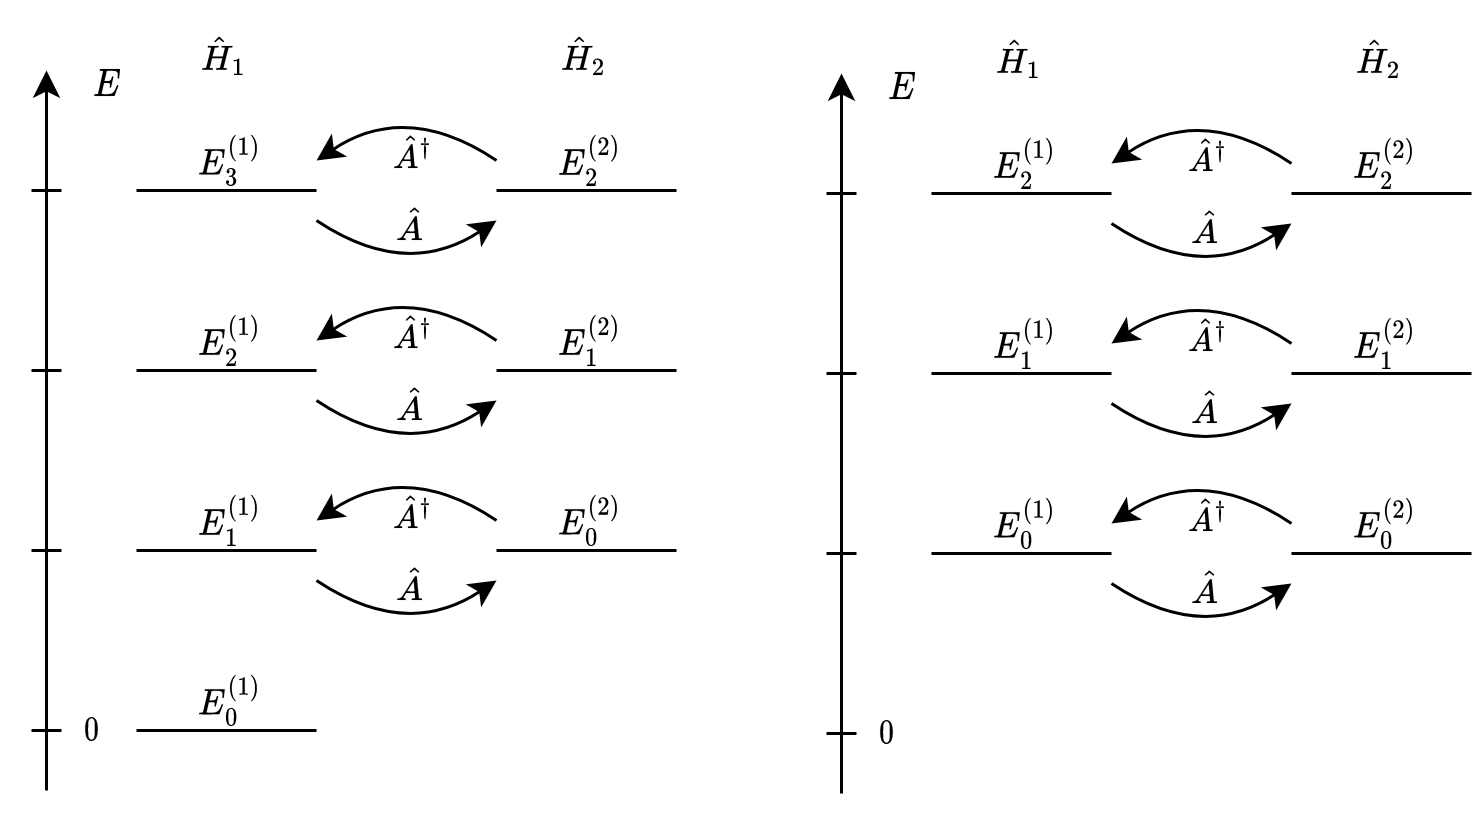
\includegraphics[width = \linewidth]{./SUSY_levels.png}
    \caption{\footnotesize Diagram illustrating the energy levels of $\hat H_1$, $\hat H_2$
    in case of unbroken and broken Supersymmetry (on the left
    and right, respectively) and the operators
    relating their respective eigenfunctions: unbroken Supersymmetry
    is characterized by the $E_0^{(1)}=0$ eigenstate.}
\end{figure}

\textbf{Note} From this point onwards Supersymmetry is considered to be unbroken,
unless otherwise specified.
\section{Example: the infinite square well}
\label{sec:square_well}
Given a simply solvable potential $V_1(x)$, its partner potential $V_2(x)$ can be found
and exactly solved: from this second potential a third ($V_3(x)$) can be derived and so on:
in this section this method is demonstrated beginning from the infinite square well potential.\\

 Consider the potential
$$V_1(x)=\begin{dcases}
-\frac{\pi^2\hbar^2}{2mL^2}&\text{if } 0\leq x\leq L\\
\infty&\text{otherwise}
\end{dcases}.
$$
This is the well known infinite square well potential, with an offset so that its ground state
has $E^{(1)}_0=0$: its energy eigenvalues and corresponding eigenstates are
$$\begin{aligned}
E^{(1)}_n = \frac{\pi^2\hbar^2}{2mL^2}n(n+2),\\
  \psi^{(1)}_n(x)=\sqrt{\frac{2}{L}}\sin\left(\frac{(n+1)\pi x}{L}\right)  
\end{aligned}
\quad\text{with }n=0,1,2,3...$$
Since Supersymmetry is unbroken, the superpotential can be found using equation
(\ref{eq:W_ground}):
$$W(x)= -\frac{\hbar}{\sqrt{2m}}\frac{\psi'^{(1)}_0(x)}{\psi^{(1)}_0(x)} = 
-\frac{\hbar}{\sqrt{2m}}\frac{\frac{\pi}{L}\cos\left(\frac{\pi x}{L}\right)}
{\sin\left(\frac{\pi x}{L}\right)}=-\frac{\hbar\pi}{L\sqrt{2m}}\cot\left(\frac{\pi x}{L}\right)
$$
then, from equation (\ref{eq:V_2}), the partner potential to $V_1(x)$ is
\begin{gather*}
V_2(x) = W^2(x)+\frac{\hbar}{\sqrt{2m}}W'(x)=
\frac{\pi^2\hbar^2}{2mL^2}\left[\cot^2\left(\frac{\pi x}{L}\right) +
\csc^2\left(\frac{\pi x}{L}\right)\right] =\\= \frac{\pi^2\hbar^2}{2mL^2}\left[
2\csc^2\left(\frac{\pi x}{L}\right)-1\right].
\end{gather*}

 Using the properties of superymmetric partner potentials, the energy spectrum of
$\hat H_2$ is readily determined:
$$E^{(2)}_n=E^{(1)}_{n+1}=\frac{\pi^2\hbar^2}{2mL^2}(n+1)(n+3)\quad \text{with }n=0,1,2,3...$$
as said before, the $E=0$ eigenstate exists only for $\hat H_1$.\\

 The eigenfunctions of $\hat H_2$ can be analytically determined with equation
(\ref{eq:A}): the ground state of $\hat H_2$ is
$$\psi^{(2)}_0(x)=\frac{1}{\sqrt{E^{(1)}_1}}\hat A\psi^{(1)}_1 = \frac{1}{\sqrt{E^{(1)}_1}}\left[
\frac{\hbar}{\sqrt{2m}}\dv[]{}{x}+W(x)\right]\psi^{(1)}_1(x)=-2\sqrt{\frac{2}{3L}}\sin^2
\left(\frac{\pi x}{L}\right),$$
with eigenvalue $E^{(2)}_0 = \frac{3\pi^2\hbar^2}{2mL^2}$.\\
 The first excited state of $\hat H_2$ is
$$\psi^{(2)}_1(x)=\frac{1}{\sqrt{E^{(1)}_2}}\hat A\psi^{(1)}_2 = -\frac{2}{\sqrt{L}}
\sin\left(\frac{\pi x}{L}\right)\sin\left(\frac{2\pi x}{L}\right),$$
with eigenvalue $E^{(2)}_1=\frac{8\pi^2\hbar^2}{2mL^2}.$\\

The complete derivation of these wavefunctions can be found in Appendix
\ref{app:square_wave}.\\

This process can be iterated: the potential $V_2(x)$ can be redefined so that
its ground state energy is $0$, a new superpotential $W_2(x)$ can be determined and from this
arises a third potential $V_3(x)$, supersymmetric partner of $V_2(x)-E^{(2)}_0$, with the same
energy spectrum,
except for the $E=0$ eigenvalue; using the new superpotential, the eigenfunctions of $\hat H_3$
can be analytically determined in a similar fashion as before.
%\footnote{forse graficino??}.
\\

This shows that, using the properties of supersymmetric partner potentials, an entire class of
analytically solvable potentials can be constructed starting from an analytically solved problem.

\section{Radial potentials}
The formalism of Supersymmetry can be easily applied to 3-dimensional radial potentials:
as is well known, if a potential $V(r,\vartheta,\varphi)$ is independent of the angular
coordinates, the eigenstates of the Hamiltonian can be factored in
$$\psi_{nlm}(r,\vartheta,\varphi) = \frac{1}{r}R_{nl}(r)Y_{lm}(\vartheta,\varphi),$$
where $Y_{lm}$ are the spherical harmonics and the reduced radial wavefunction $R_{nl}(r)$
satisfies
$$- \dv[2]{R_{nl}}{r}+\left[V(r)+\frac{l(l+1)}{r^2}\right]R_{nl}(r)=ER_{nl}(r),$$
in units where $\hbar=2m=1$.\\
This is a 1-dimensional Schrödinger equation with an effective potential that incorporates
the angular momentum barrier.

\subsection{Example: Oscillator potential}
Consider the superpotential
\begin{equation}
W(r) = \frac{\omega r}{2}-\frac{l+1}{r}:
\label{eq:osc_superpot}
\end{equation}
its associated partner potentials are
\begin{equation}
\begin{dcases}
V_1(r)=\frac{\omega^2r^2}{4}+\frac{l(l+1)}{r^2}-\left(l+\frac{3}{2}\right)\omega\\
V_2(r)=\frac{\omega^2r^2}{4}+\frac{(l+1)(l+2)}{r^2}-\left(l+\frac{1}{2}\right)\omega
\label{eq:osc_pot}
\end{dcases}.
\end{equation}
The potential $V_1(r)$ is the effective potential for the isotropic harmonic oscillator: its
$l$'th partial wave has the $l+1$'th partial wave of the same potential as its supersymmetric
partner. This radial potential will be used later as an example of the advantages of the 
supersymmetric approach.

\section{Transmission and reflection coefficients}
Another implication of the properties of supersymmetric Quantum Mechanics is the relationship
between transmission and reflection coefficients of two partner potentials in scattering
problems: before deriving it, it is necessary to establish the conditions on $W(x)$ that
guarantee the existence of unbound eigenstates.\\

 Consider the usual partner potentials $V_1(x)$ and $V_2(x)$, in units where
$\hbar =2m=1$:
\begin{gather*}
V_1(x)=W^2(x)-W'(x)\\
V_2(x)=W^2(x)+W'(x).
\end{gather*}
The corresponding Hamiltonians $\hat H_1$, $\hat H_2$ admit unbound eigenstates if and only if
$$\lim\limits_{x\to\pm\infty}V_i(x) = L^{(i)}_\pm\in\mathbb{R},$$
and the only way for $V_i(x)$ to have finite limits at infinity is if
$$\lim\limits_{x\to\pm\infty}W(x) = W_\pm\in\mathbb{R}
\iff\lim\limits_{x\to\pm\infty}V_i(x)=W^2_\pm.$$
Under this condition on $W(x)$, the partner Hamiltonians admit unbound eigenstates.

Consider a progressive plane wave of energy $E$ scattering on the potential $V_i(x)$: the
wavefunctions $\psi^{(i)}(x)$ will have limits
$$\begin{dcases*}
      \lim\limits_{x\to-\infty} \psi^{(i)}(x) = e^{ikx}+R_ie^{-ikx}\\
      \lim\limits_{x\to+\infty} \psi^{(i)}(x) = T_ie^{ik'x}
  \end{dcases*}\text{, with}\quad
\begin{aligned}
    k = \sqrt{E-W^2_{-}}\\
    k'= \sqrt{E-W^2_{+}}
\end{aligned},$$
where $R_i$ are the \textit{reflection coefficients} and $T_i$ the \textit{transmission
coefficients} of the two potentials.

 Applying property (\ref{eq:A+}) in the limit $x\to-\infty$ yields
\begin{gather*}
e^{ikx}+R_1e^{-ikx} = N\left[-\dv[]{}{x}e^{ikx}+W_-e^{ikx} + R_2\left(
-\dv[]{}{x}e^{-ikx}+W_-e^{-ikx}\right)\right]=\\
=Ne^{ikx}(-ik+W_-)+Ne^{-ikx}(ik+W_-)R_2:
\end{gather*}
equating the coefficients of the exponentials
\begin{equation}
\begin{dcases*}
R_1=N(W_-+ik)R_2\\
N=\frac{1}{W_--ik}
\end{dcases*} \iff R_1 = \frac{W_-+ik}{W_--ik}R_2.
\label{eq:refl}
\end{equation}
Applying the same property to the limit $x\to+\infty$ gives
$$T_1e^{ik'x} = N\left(-\dv[]{}{x}+W_+\right)e^{ik'x}T_2 = N(W_+-ik')T_2,$$
and it follows that
\begin{gather}
T_1 = \frac{W_+-ik'}{W_--ik}T_2.
\label{eq:trans}
\end{gather}
 These two relations imply
\begin{gather*}
|R_1|^2 = |R_2|^2\\
|T_1|^2 = |T_2|^2,
\end{gather*}
which means the transmission and reflection probabilities are the same for both partner
potentials: this result is important, especially in more than 1 dimension, as it relates the
$S$-matrices of different scattering problems.
\section{Example: Reflectionless potentials}
\label{sec:refl1}
In this section the relationship between the transmission and reflection coefficients of partner
Hamiltonians will be used to construct a family of algebraically solvable potentials, starting
from the free particle, which has reflection coefficient $R=0$.

Consider the superpotential
$$W(x;B)=B\tanh(x)$$
and its partner potentials
\begin{gather*}
    V_1(x;B)=B^2-B(B+1)\cosh^{-2}(x)\\
    V_2(x;B)=B^2-B(B-1)\cosh^{-2}(x).
\end{gather*}
Both potentials have finite limits, because
\begin{gather*}
\lim\limits_{x\to\pm\infty}W(x;B)=\pm B\\
\lim\limits_{x\to\pm\infty}V_i(x;B)=B^2,
\end{gather*}
so they always admit unbound eigenstates with $E\geq B^2$.\\

Consider $B=1$: the superpotential and potentials are
\begin{gather*}
W(x;B=1)=\tanh(x)\\
\begin{dcases*}
    V_1(x;B=1)=1-2\cosh^{-2}(x)\\
V_2(x;B=1)=1
\end{dcases*}
\end{gather*}
It is clear that $\hat H_2(B=1)$ is the Hamiltonian of a free particle, so its transmission and
reflection coefficients are
$$
\begin{dcases*}
T_2(k;B=1)=1\\
R_2(k;B=1)=0.
\end{dcases*}
$$
Then, from equations (\ref{eq:refl}) and (\ref{eq:trans}), it follows that the coefficients for
$H_1$ are
$$
\begin{dcases*}
T_1(k;B=1)=\frac{1-ik}{-1-ik}\\
R_1(k;B=1)=0
\end{dcases*}.
$$
Using (\ref{eq:ground_state}), the ground state wavefunction is
$$\psi^{(1)}_0(x;B=1)=N\exp\left[-\int_{x_0}^{x}\dd y\tanh(y)\right]=N\cosh^{-1}(x)$$
and it is normalizable: from the properties discussed before, this
implies that Supersymmetry is unbroken, so $\hat H_1(B=1)$ admits exactly one bound
state with $E^{(1)}_0(B=1)=0$ and a continuum of unbound states with
$E^{(1)}(B=1)\geq1$.\\

Consider now $B=2$, the two potentials are
$$\begin{dcases*}
    V_1(x;B=2)=4-6\cosh^{-2}(x)\\
V_2(x;B=2)=4-2\cosh^{-2}(x)
\end{dcases*}
$$
and it is clear that $V_2(x;B=2)$ differs from $V_1(x;B=1)$ just by a constant, so its
transmission and reflection coefficients must be the same (and their eigenfunctions are
proportional to one another); using once again equations (\ref{eq:refl}) and (\ref{eq:trans}),
the transmission coefficient of $\hat H_1(B=2)$ is
$$
T_1(k;B=2)=\frac{2-ik}{-2-ik}\frac{1-ik}{-1-ik}
$$
and its ground state wavefunction is
$$\psi^{(1)}_0(B=2)=N\cosh^{-2}(x)$$
so Supersymmetry must again be unbroken and $E^{(1)}_0(B=2)=0$; it is also clear that
$\hat H_2(B=2)$ admits a bound state with $E^{(2)}_0(B=2)=3$ (its ground state), and so does
$\hat H_1(B=2)$: the corresponding eigenfunction is
\begin{gather*}
\psi^{(1)}_1(x;B=2)=\hat A^{\dagger}(B=2)\psi^{(2)}_0(x;B=2)=\\
=\hat A^\dagger(B=2)\psi^{(1)}_0(x;B=1)=N\tanh(x)\cosh^{-1}(x),
\end{gather*}
where the first equality is due to the properties of partner Hamiltonians and the second
is due to the fact that $V_2(B=2) = V_1(B=1)+3$.\\

This process can be iterated: $\forall B=p\in\mathbb{N}$, the potentials $V_2(x;p)$ are
reflectionless (as they differ from $V_1(x;p-1)$ just by a constant and so on),
and so are $V_1(x;p)$, as they are partner potentials; their transmission coefficients are
$$T_1(k;p)=\frac{(p-ik)(p-1-ik)...(1-ik)}{(-p-ik)(-p+1-ik)...(-1-ik)}=
\frac{\Gamma(-p-ik)\Gamma(p+1-ik)}{\Gamma(-ik)\Gamma(1-ik)},$$
their ground state wavefunctions are
$$\psi_0^{(1)}(x;p)=N\exp\left[-p\int_{x_0}^{x}\dd y\tanh(y)\right]=N\cosh^{-p}(x),$$
the first excited state wavefunctions are
$$\psi^{(1)}_1(x;p)=\hat A^\dagger(p)\psi_0^{(1)}(x;p-1)=N\tanh(x)\cosh^{1-p}(x)
$$
and finally the $q$'th excited state ($0<q<p$, as they admit $p$ bound states) can be determined
from the $q-1$'th as
$$\psi^{(1)}_q(x;p) = \hat A^\dagger(p)\psi^{(2)}_{q-1}(x;p)=
\hat A^\dagger(p)\psi^{(1)}_{q-1}(x;p-1),$$
as can be deduced from Figure \ref{fig:reflectionless}.
\begin{figure}[H]
    \centering
    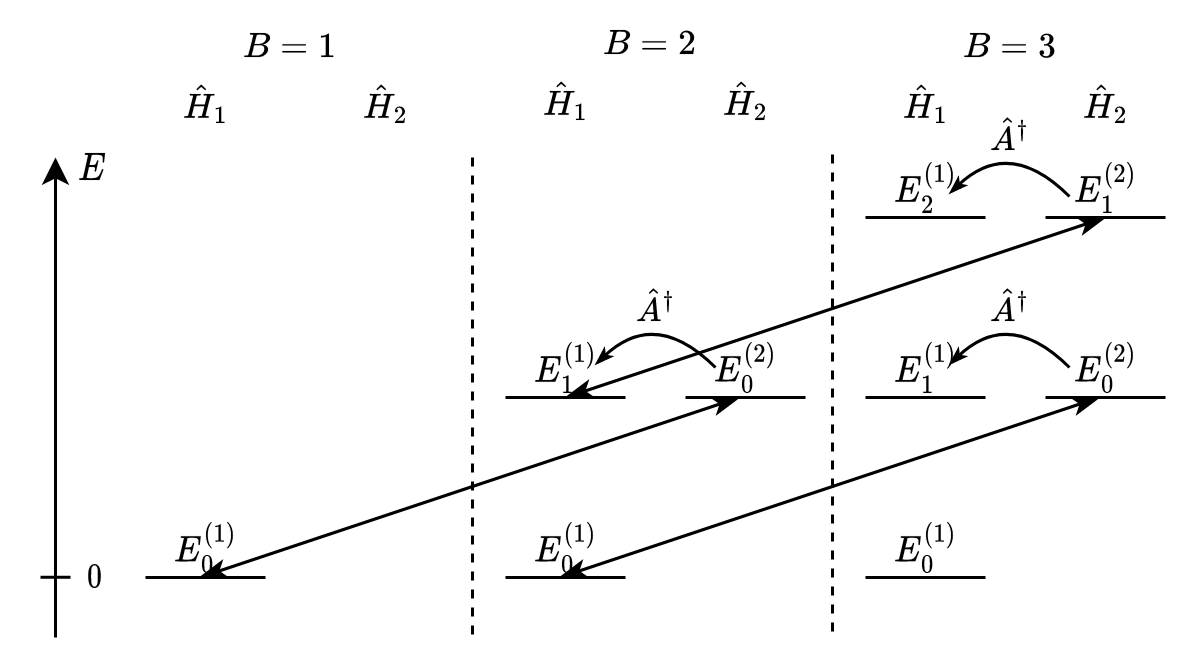
\includegraphics[width = \linewidth]{./reflectionless.png}
    \caption{\small Diagram for the construction of the bound excited states of
    $\hat H_1(B\leq3)$: the equality of the wavefunctions (save normalization) is depicted as a
    double arrow, while the use of the operator $\hat A^\dagger$ with a single arrow.
    The distribution of the levels is not to scale.}
    \label{fig:reflectionless}
\end{figure}

Using the properties of Supersymmetry, it was possible to construct a family of reflectionless
potentials and easily compute their transmission coefficients and bound state wavefunctions, as
they are all related to the free particle Hamiltonian.\\

In this example a more fundamental underlying property that relates the Hamiltonians
$\hat H_i(B)$ to one another, called \textit{shape invariance}, is at work: it will
be discussed more thoroughly in the next chapter.

%------------------------------------------------------------------------------------------------
\newpage
\chapter{Shape Invariance}
\thispagestyle{empty}
This chapter will introduce a stricter condition on supersymmetric partner potentials, called
\textit{shape invariance}: the intuition behind this concept is the fact that certain
potentials resemble one another and differ only in the choice of fixed parameters
and/or constant energy offsets.

Here the formalization is presented and it is proven that this condition is
a sufficient hypothesis to devise a generalization of the ladder operators, normally
employed in the solution of the quantum harmonic oscillator; finally, some applications
will be discussed in detail.
\section{Definition and fundamental properties}
\begin{defn}
Two supersymmetric partner potentials,
\begin{gather*}
V_1(x;a_1) = W'(x;a_1) - W^2(x;a_1)\\
V_2(x;a_1) = W'(x;a_1) + W^2(x;a_1),
\end{gather*}
dependent from a set of parameters $a_1$, are called \textit{shape invariant} if and only if
\begin{equation}
V_2(x;a_1) = V_1(x;a_2)+R(a_1),
\label{eq:SIP}
\end{equation}
where $a_2 = f(a_1)$ and $R(a_1)$ does not depend on $x$.
\label{def:SIP}
\end{defn}
From this definition follows the fundamental property of shape invariant potentials:
adding the kinetic operator to equation (\ref{eq:SIP}) gives
$$\hat H_2(a_1) = \hat H_1(a_2)+R(a_1)\longrightarrow\hat H_1(a_2) = \hat H_2(a_1)-R(a_1).$$
Since the Hamiltonians differ by a constant, their eigenfunctions must be proportional to
one another and the corresponding energy eigenvalues must differ only by the constant
$R(a_1)$:
%using the ground state of $\hat H_1(a_2)$ implies that,
if Supersymmetry is unbroken,
the ground state energy for $\hat H_2(a_1)$ is then known to be
$$E^{(2)}_0(a_1) = E^{(1)}_0(a_2)+R(a_1)=R(a_1)$$
and the ground states of $\hat H_1(a_2)$ and $\hat H_2(a_1)$ are proportional
$$\psi^{(1)}_0(x;a_2)=\psi^{(2)}_0(x;a_1)=N\exp\left[-\int_{x_0}^{x}\dd y W(y;a_2)
\right].$$
From the properties of Supersymmetry follows that
$$\psi_1^{(1)}(x;a_1)=\hat A^\dagger(a_1)\psi^{(2)}_0(x;a_1)\Rightarrow
\psi^{(1)}_1(x;a_1)=\hat A^\dagger(a_1)\psi^{(1)}_0(x;a_2).$$
Since the function $f$ that relates $a_2=f(a_1)$ is known, the shape invariance condition
implies a relationship between the ground state wavefunction and the first excited state!
This process can be generalized to construct \textit{all} bound states of $\hat H_1(a_1)$.
\section{Generalized ladder operator method}
To generalize the relationship found in the previous section, a family of Hamiltonians must be
constructed from two supersymmetric partner potentials and
the function $f$, which completely determines the shape invariance:
starting from the partner potentials $V_1(x;a_1)$ and $V_2(x;a_1)$, 
consider the family of potentials
\begin{equation}
V_s(x;a_1):=V_1(x;a_s)+\sum_{k=1}^{s-1}R(a_k),\text{with }s=1,2...
\label{eq:SIP_family}
\end{equation}
where
$$a_s = f^{s-1}(a_1).$$
\begin{thm}
    \textit{The potentials $V_s(x;a_1)$ and $V_{s+1}(x;a_1)$ are shape invariant potentials
    $\forall s=1,2...$}
\end{thm}
\textbf{Proof} The base case $s=1$ follows from definition \ref{def:SIP}.\\
For $s>1$, let $b=a_s$: the potential $V_{s+1}(x;a_1)$ can be expressed as
$$V_{s+1}(x;a_1)=V_1(x;f(b))+\sum_{k=1}^{s-1}R(a_k)-R(b),$$
using equation (\ref{eq:SIP}) with $a_1:=b$ yields
$$V_{s+1}(x;a_1) = V_2(x;b)+\sum_{k=1}^{s-1}R(a_k).$$
Since
$$V_s(x;a_1) = V_1(x;b)+\sum_{k=1}^{s-1}R(a_k),$$
$V_s(x;a_1)$ and $V_{s+1}(x;a_1)$ are respectively equal to $V_1(x;a_1)$ and $V_2(x;a_1)$, save
a constant offset, so they are in turn supersymmetric partners and shape invariant
potentials.\qed\\

 Adding the kinetic operator provides a family of Hamiltonians
$$\hat H_s(a_1) = -\dv[2]{}{x} + V_1(x;a_s) + \sum_{k=1}^{s-1}R(a_k),$$
in which $\hat H_s$ and $\hat H_{s+1}$ are supersymmetric partners.\\
They can also be expressed in terms of $\hat H_1$ and $\hat H_2$:
\begin{gather*}
\hat H_s(a_1) = \hat H_1(a_s)+\sum_{k=1}^{s-1}R(a_k)\\
\hat H_{s+1}(a_1) = \hat H_2(a_s)+\sum_{k=1}^{s-1}R(a_k).
\end{gather*}
Ignoring normalizations, this implies that the operators
\begin{gather*}
\hat A_s := \hat A(a_s)\\
\hat A_s^\dagger :=\hat A^\dagger(a_s)
\end{gather*}
relate their eigenfunctions just like $\hat A(a_1), \hat A^\dagger(a_1)$ relate those of
$\hat H_1(a_1), \hat H_2(a_1)$.\\

If $\hat H_1$ admits $p$ bound states, then $\hat H_s$ admits $p-s$ bound states, so it is clear
that this process can be iterated at most $s=p-1$ times.

 Using this method, the energy eigenvalues for $V_1(x;a_1)$ can be recursively
determined: the ground state energy, if Supersymmetry is unbroken, is
$$E_0^{(1)}(a_1)=0,$$
the first excited state's is
$$E_1^{(1)}(a_1) = E_0^{(2)}(a_1) = E_0^{(1)}(a_2)+R(a_1)=R(a_1),$$
where the first equality follows from Supersymmetry and the second from the shape invariance;
the second excited state's is
\begin{gather*}
E_2^{(1)}(a_1)=E_1^{(2)}(a_1)=E_0^{(3)}(a_1)=E_0^{(2)}(a_2)+R(a_1)=\\
= E_0^{(1)}(a_3)+R(a_1)+R(a_2)=R(a_1)+R(a_2).
\end{gather*}
Iterating this process shows that the $n$'th excited state (with $0<n\leq p$) has energy
\begin{equation}
E_n^{(1)}(a_1) = \sum_{k=1}^{n}R(a_k),
\label{eq:SIP_spectrum}
\end{equation}
and, since $\hat H_s(a_1)$ is a family of supersymmetric partners, this is also the ground state
energy for $\hat H_{n+1}(a_1)$:
$$E_{0}^{(n+1)}(a_1) = E^{(1)}_n(a_1).$$

This method also provides an algebraic expression for the energy eigenfunctions of $V_1(x;a_1)$:
since Supersymmetry is unbroken, the ground state wavefunction is
$$\psi^{(1)}_0(x;a_1)=N\exp\left[-\int_{x_0}^{x}\dd yW(y;a_1)\right].$$
Using, respectively, Supersymmetry and shape invariance and ignoring
normalization, the first excited state's wavefunction
is
$$\psi^{(1)}_1(x;a_1) =\hat A^\dagger_1\psi^{(2)}_0(x;a_1)=
\hat A^\dagger_1\psi^{(1)}_0(x;a_2)$$
and the second excited state's is
$$\psi_2^{(1)}(x;a_1)=\hat A^\dagger_1\psi_1^{(2)}(x;a_1)
= \hat A^\dagger_1 \hat A^\dagger_2\psi_0^{(3)}(x;a_1).$$
Using the shape invariance conditions
$$\psi_0^{(3)}(x;a_1)=\psi_0^{(2)}(x;a_2)=\psi_0^{(1)}(x;a_3)$$
yields
$$\psi^{(1)}_2(x;a_1)= \hat A^\dagger_1\hat A^\dagger_2\psi_0^{(1)}(x;a_3).$$
Iterating this line of reasoning, the $n$'th excited state's wavefunction is
\begin{equation}
\psi^{(1)}_n(x;a_1)=\hat A^\dagger_1...\hat A^\dagger_{n}\psi^{(1)}_0(x;a_{n+1}),
\label{eq:SIP_wave}
\end{equation}
or
\begin{equation}
    \psi^{(1)}_n(x;a_1)=\hat A_1^\dagger\psi^{(1)}_{n-1}(x;a_2),
    \label{eq:SIP_wave_rec}
\end{equation}
which effectively is a generalization of the ladder operators for the quantum harmonic
oscillator, since the function $f$ that relates the parameters is known.
\section{Example: Reflectionless potentials}
As stated at the end of \ref{sec:refl1}, the family of reflectionless potentials
associated with the partner potentials
\begin{equation}
    \begin{dcases}
	V_1(x;B)= B^2-B(B+1)\cosh^{-2}(x)\\
	V_2(x;B)= B^2-B(B-1)\cosh^{-2}(x)
	\label{eq:v12refl}
    \end{dcases}\text{, with }
    W(x;B)=B\tanh(x)
\end{equation}
is also a family of shape invariant potentials: in this section the same results
will be found using this property, in addition to the full energy spectra of the
Hamiltonians.\\

Consider the potentials (\ref{eq:v12refl}): it is easy to show that
$$V_2(x;B)=V_1(x;B-1)+B^2-(B-1)^2,$$
so $V_1$ and $V_2$ are shape invariant potentials with
\begin{align*}
&a_1:=B,\\
&a_2=f(a_1=B):=B-1,\\
&R(a_1=B):=B^2-(B-1)^2 = a_1^2-a_2^2.
\end{align*}
Since $f$ is a simple translation, $a_n$ is readily computed to be
$$a_n = f^{n-1}(a_1=B)=B-n+1,$$
and so is $R(a_k)$:
$$R(a_k) = a_k^2-a_{k+1}^2.$$
With these quantities, it is easy to apply the properties found in the previous section:
Supersymmetry is unbroken, since the ground state wavefunction (\ref{eq:ground_state})
$$\psi^{(1)}_0(x;B) = N\exp\left[-B\ln\left(\cosh(x)\right)\right]=N\cosh^{-B}(x)$$
is normalizable, so the ground state energy must be $E_0^{(1)}(B)=0$.

 The other energy eigenvalues are immediately determined from equation
(\ref{eq:SIP_spectrum}):
$$E_n^{(1)}(B) = \sum_{k=1}^{n}R(a_k) = a_1^2-a_2^2+a^2_2-...-a_{n+1}^2 =
a_1^2-a_{n+1}^2=B^2-(B-n)^2.$$
These eigenvalues could not be determined as easily without the shape invariance condition.\\

To determine the eigenfunctions, consider first the operator $\hat A^\dagger_s$
earlier defined
\begin{gather*}
\hat A_s^\dagger = \hat A^\dagger(a_s) = - \dv[]{}{x} + W(x;a_s) = -\dv[]{}{x}+(B-s+1)\tanh(x).
\end{gather*}
The ground state eigenfunction was already determined to be
$$\psi_0^{(1)}(x;B) = N\cosh^{-B}(x),$$
so, using equation (\ref{eq:SIP_wave_rec}), the first excited state's wavefunction is
$$\psi_1^{(1)}(x;B)=\left[-\dv[]{}{x}+B\tanh(x)\right]\cosh^{1-B}(x)=
N\tanh(x)\cosh^{1-B}(x),$$
the second's is
$$\psi_2^{(1)}(x;B)=\left[-\dv[]{}{x}+B\tanh(x)\right]\tanh(x)\cosh^{2-B}(x)$$
and so on.
\section{Example: Radial Oscillator potential}
Consider the radial superpotential (\ref{eq:osc_superpot})
$$W(r;l;\omega)=\frac{\omega r}{2}-\frac{l+1}{r}$$
and its associated partner potentials
\begin{equation*}
\begin{dcases}
V_1(r;l;\omega)=\frac{\omega^2r^2}{4}+\frac{l(l+1)}{r^2}-\left(l+\frac{3}{2}\right)\omega\\
V_2(r;l;\omega)=\frac{\omega^2r^2}{4}+\frac{(l+1)(l+2)}{r^2}-\left(l+\frac{1}{2}\right)\omega
\end{dcases}:
\end{equation*}
it is easy to show that they are also shape invariant potentials, as
$$V_2(r;l;\omega) = V_1(r;l+1;\omega)+2\omega,$$
in this case
\begin{align*}
&a_1:=l,\\
&a_2=f(a_1=l):=l+1.
\end{align*}
As in the first example, the function $f$ is just a translation, so
\begin{align*}
&a_k=f^{k-1}(a_1)=l+k-1,\\
&R(a_k):=2\omega\quad\forall k=1,2...
\end{align*}
As always, its ground state radial wavefunction can be determined from (\ref{eq:ground_state}):
\begin{gather*}
    R_{0}^{(1)}(r;l;\omega)=N\exp\left[-\int_{r_0>0}^{r}\dd\rho\frac{\omega\rho}{2}-
    \frac{l+1}{\rho}\right]= N r^{l+1}\exp\left[-\frac{\omega}{4}r^2\right],
\end{gather*}
so the $E^{(1)}_0(l;\omega)=0$ eigenfunctions are
$$\psi^{(1)}_{0lm}(r,\vartheta,\varphi)=\mathcal{N}r^{l}\exp\left[-\frac{\omega}{4}r^2\right]
Y_{lm}(\vartheta,\varphi).$$
Since this wavefunction is normalizable, Supersymmetry is unbroken, so $E_0^{(1)}(l;\omega)=0$
and, using (\ref{eq:SIP_spectrum}), the other energy eigenvalues are immediately determined to be
$$E_n^{(1)}(l;\omega)=\sum_{k=1}^{n}2\omega=2n\omega.$$
The excited states' wavefunctions can be determined using equation (\ref{eq:SIP_wave_rec})
recursively:
\begin{gather*}
R^{(1)}_{1}(r;l;\omega)=\hat A^\dagger(l;\omega)R^{(1)}_{0}(r;l+1;\omega)=N\left(
-\dv[]{}{r}+\frac{\omega}{2}r-\frac{l+1}{r}\right)r^{l+2}\exp\left[-\frac{\omega}{4}r^2\right],
\end{gather*}
which yields
$$R_1^{(1)}(r;l;\omega)=N\left(\omega r^2-2l-3\right)r^{l+1}\exp\left[-\frac{\omega}{4}r^2
\right],$$
so the $E^{(1)}_1(l;\omega)$ eigenfunctions are
$$\psi_{1lm}(r,\vartheta,\varphi) = \mathcal{N}(\omega r^2-2l-3)r^{l}\exp
\left[-\frac{\omega}{4}r^2\right]Y_{lm}(\vartheta,\varphi).$$
%\textbf{NOTE TO SELF} ci sono delle cose che non mi quadrano: non appaiono costrizioni su $l$,
%quindi c'è degenerazione nello stato fondamentale (che è impossibile!). 
%\href{https://en.wikipedia.org/wiki/Quantum_harmonic_oscillator#Example:_3D_isotropic_harmonic_oscillator}{Pagina di Wikipedia}: sarebbe bello far vedere che emergono anche da qui, se no
%questo metodo non è una vera alternativa a una soluzione analitica (polinomi di Laguerre
%generalizzati).\\

The purpose of this example is to show that a supersymmetric approach to a familiar problem
can result in an elegant and brief algebraic solution.
\COMMENT{
TODOLIST
- esempi reflectionless OK
- parte 3D e potenziale oscillante OK
- SIP OK
- SWKB
}
\newpage

%--------------------------------------------------------------------------------------
\thispagestyle{empty}
\chapter{Supersymmetric WKB}
The Wentzel–Kramers–Brillouin (WKB) approximation is a well known method of finding
asymptotic series in powers of $\hbar$ for the energy eigenvalues and eigenfunctions
of Schrödinger's equation: for bound states in a generalized potential well $V(x)$
which obeys the WKB condition
$$\left|\frac{\hbar p'(x)}{p^2}\right| =
\left|\frac{\hbar m\pdv[]{V}{x}}{p^3}\right|<<1\text{, where}
\; p(x):=\sqrt{2m\left[E-V(x)\right]}$$
i.e. slowly varying potentials and high momentum, the first semi-classical
correction yields a quantization condition for the first order of the energy
eigenvalues
\begin{equation}
\int_{x_1}^{x_2}\dd y \sqrt{2m\left[E_n-V(y)\right]}=\left(n+\frac{1}{2}\right)
\hbar\pi,
\label{eq:WKB_quant}
\end{equation}
with $V(x_1) = V(x_2) = E_n$.
It will be shown that this condition can yield more precise results using a
supersymmetric approach called the SWKB approximation.

\textbf{Note} In this chapter the $\hbar$ and $m$ dependencies of the potentials
will be explicit, since they are necessary for the WKB approximation.
\section{Lowest order SWKB: unbroken Supersymmetry}
Consider two supersymmetric partner potentials
$$
\begin{dcases*}
V_1(x) = W^2(x)-\frac{\hbar}{\sqrt{2m}}W'(x)\\
V_2(x) = W^2(x)+\frac{\hbar}{\sqrt{2m}}W'(x)
\end{dcases*}
$$
so that, formally, $W(x) = O(\hbar^0)$ and
$\hbar W'(x) = O(\hbar)$: the condition (\ref{eq:WKB_quant}) for $V_1$
is
$$\int_{x_1}^{x_2}\dd y\sqrt{2m\left[E^{(1)}_n-W^2(y)+\frac{\hbar}{\sqrt{2m}}W'(y)
\right]}=\left(n+\frac{1}{2}\right)\hbar\pi;
$$
expanding the integrand in powers of $\hbar$ yields
$$\sqrt{2m\left(E_n^{(1)}-W^2(y)\right)}+\frac{\hbar}{2}\frac{W'(y)}{\sqrt{E-W^2(y)}}+
O(\hbar^2),$$
the condition $V_1(x_1)=V_1(x_2)=E^{(1)}_n$ must be truncated at $O(\hbar^0)$
and so becomes
$$W^2(a)=W^2(b)=E_n^{(1)}\text{, where }
x_1 = a + O(\hbar),\;x_2 = b + O(\hbar).$$
The condition (\ref{eq:WKB_quant}) becomes
$$\int_{a}^{b}\dd y \sqrt{2m\left(E_n^{(1)}-W^2(y)\right)}+\frac{\hbar}{2}
\int_{a}^{b}\dd y \frac{W'(y)}{\sqrt{E^{(1)}_n-W^2(y)}}=\left(n+\frac{1}{2}\right)
\hbar\pi,$$
the second integral is elementar and its value is
$$\eval{\arcsin\left(\frac{W(y)}{\sqrt{E^{(1)}_n}}\right)}_a^b.$$
Supposing Supersymmetry is unbroken, conditions (\ref{eq:lim_W}) imply
$$-W(a)=W(b)=\sqrt{E^{(1)}_n}$$
that is
$$\eval{\arcsin\left(\frac{W(y)}{\sqrt{E^{(1)}_n}}\right)}_a^b=\pi.$$
So, with the hypothesis of unbroken Supersymmetry, the first order SWKB
quantization condition on $V_1(x)$ is
\begin{equation}
\int_{a}^{b}\dd y \sqrt{2m\left(E^{(1)}_n-W^2(y)\right)} = n\hbar\pi.
\label{eq:SWKB_quant_V1}
\end{equation}
The calculations for $V_2(x)$ are exactly the same, save a negative sign before the
$O(\hbar)$ term: its SWKB quantization condition is
\begin{equation}
\int_{a}^{b}\dd y \sqrt{2m\left(E^{(2)}_n-W^2(y)\right)} = (n+1)\hbar\pi.
\label{eq:SWKB_quant_V2}
\end{equation}
The advantages of this method are immediately clear: since the integrand
is strictly positive $\forall y\in[a,b]$, the quantization condition of $V_1$
with $n=0$ implies that the extrema of integration must coincide, so
$$W(a)=-W(b)=-W(a)=0=\sqrt{E^{(1)}_0}:$$
the ground state eigenvalue is exactly known to be
$E^{(1)}_0=0$ just from the first $\hbar$ order; moreover, these approximations
for the eigenvalues of the partner potentials respect the fundamental property of 
supersymmetric partner potentials $E^{(1)}_{n+1}=E^{(2)}_n$.

\textbf{Note} The regular WKB approximation yields better results the
greater is $n$, but this supersymmetric method is also exact for the ground state
energy: given this other constraint, it is natural to think that the SWKB method
will be, in general, a better approximation in the case of unbroken Supersymmetry.

\section{Lowest order SWKB: broken Supersymmetry}
The derivation of the new quantization condition for broken supersymmetry
is similar to the one for unbroken supersymmetry, with the key difference being
that at the $O(\hbar^0)$ turning points the superpotential must have the same
sign, as discussed after the definition of unbroken Supersymmetry:
$$W(a) = W(b) = \sqrt{E_n^{(1)}}$$
and so the $O(\hbar)$ integral vanishes for both $V_1$ and $V_2$, yielding
$$\int_a^b \dd y \sqrt{2m\left(E_n^{(i)}-W^2(y)\right)} = \left(n+\frac{1}{2}
\right)\hbar\pi$$\\

\textbf{Note} The reason why the SWKB method yields better results than regular
WKB for both unbroken and broken supersymmetry lies in the fact that the
factorization of supersymmetric partner Hamiltonians uncovers a term in the
potential that is $O(\hbar^1)$, that can be taken out of the quantization
condition integral and absorbed in the constant of the right hand side of the
regular WKB condition. For further discussion on broken supersymmetry,
see \cite{dutt_ref_in_ref}, as cited in \cite{cooper_main}
\section{SWKB for Shape Invariant Potentials}
This method is especially powerful for shape invariant potentials: consider the
family of potentials (\ref{eq:SIP_family})
$$V_s(x;a_1) = V_1(x;a_s) + \sum_{k=1}^{s-1}R(a_k):$$
the SWKB condition (\ref{eq:SWKB_quant_V1}) for the Hamiltonian $\hat H_1$ has the form
$$\int_{a}^{b}\dd y \sqrt{2m\left(E_n^{(1)}-W^2(y,a_s)\right)} = 
\int_{a}^{b}\dd y \sqrt{2m\left(E_n^{(s)}-\sum_{k=1}^{s-1}R(a_k)-W^2(x;a_s)\right)} = n\hbar\pi.$$
If supersymmetry is unbroken, as argued before, the quantization condition is
exact for the ground state energy
$$E^{(1)}_0 = 0 \iff E^{(s)}_0 = \sum_{k=1}^{s-1}R(a_k):$$
since all the potentials are shape invariant, this implies that the ground state energy \textit{for each
Hamiltonian} $\hat H_s$ is exact, moreover, for the properties discussed in the
previous chapter
$$E^{(s+1)}_0 = E_s^{(1)}$$
and so \textbf{all} the energy eigenvalues of ${\hat H_1}$ are exactly determined by the SWKB
quantization condition: this is a remarkable result, as the class of shape
invariant potentials is bigger than the class of known analytically solvable
potentials.




\COMMENT{
%explicit vs implicit \hbar dependency in W(x) and V_i(x), MF said it is unclear
\textbf{Note} This derivation is founded on the assumption that $W(x) =
O(\hbar^0)$ and $\hbar W'(x)=O(\hbar)$: this condition seems to imply that
this quantization condition holds only for potentials that contain an $O(\hbar)$
term, but it is always possible to absorb the $\hbar$ dependency with a choice of
dimensional parameters;
for example the superpotential for the reflectionless potentials yields
$$W(x;B) = B\tanh(x) \longrightarrow V_1(x;B) = B^2 - B(B+\hbar)\cosh^{-2}(x):$$
a choice of parameter $B$ so that $B(B+\hbar)$ is independent of $\hbar$ yields
an $O(\hbar^0)$ potential, with a constant $O(\hbar)$ energy
offset, which can always be discarded.}

\newpage
\thispagestyle{empty}
{\Huge \textbf{Appendix}}
\addcontentsline{toc}{chapter}{Appendix}
\setcounter{chapter}{4}
\addtocontents{toc}{\protect\setcounter{tocdepth}{0}}
\section{Infinte square well}
\setcounter{section}{1}
\label{app:square_wave}

Here are shown the calculations for the ground state wavefunction of the
potential $V_2$ determined in Section \ref{sec:square_well}:
\begin{align*}
&\psi^{(2)}_0(x)=\frac{1}{\sqrt{E^{(1)}_1}}\hat A\psi^{(1)}_1 = \frac{1}{\sqrt{E_1}}\left[
\frac{\hbar}{\sqrt{2m}}\dv[]{}{x}+W(x)\right]\psi^{(1)}_1(x)=\\
&=\sqrt{\frac{2mL^2}{\pi^2\hbar^2\cdot1(1+2)}}\frac{\hbar}{\sqrt{2m}}\left[\dv[]{}{x}-\frac{\pi}{L}
\cot\left(\frac{\pi x}{L}\right)\right]\sqrt{\frac{2}{L}}\sin\left(\frac{2\pi x}{L}\right) =\\
&=\sqrt{\frac{2}{3L}}\left[2\cos\left(\frac{2\pi x}{L}\right) - \frac{\cos\left(\frac{\pi x}{L}\right)}
{\sin\left(\frac{\pi x}{L}\right)}2\cos\left(\frac{\pi x}{L}\right)\sin\left(\frac{\pi x}{L}\right)\right]=
-2\sqrt{\frac{2}{3L}}\sin^2\left(\frac{\pi x}{L}\right)
\end{align*}

 The first excited state is
$$\psi^{(2)}_1(x)=\frac{1}{\sqrt{E^{(1)}_2}}\hat A\psi^{(1)}_2$$
letting $\alpha :=\frac{\pi x}{L}$ this becomes
\begin{align*}
&\psi^{(2)}_1(x)= \sqrt{\frac{2mL^2}{\pi^2\hbar^2\cdot2(2+2)}}\frac{\hbar}{\sqrt{2m}}
\left[\frac{\pi}{L}\dv[]{}{\alpha} - \frac{\pi}{L}\cot(\alpha)\right]\sqrt{\frac{2}{L}}\sin(3\alpha)=\\
&=\frac{1}{2\sqrt{L}}\left[3\cos(3\alpha)-\cot(\alpha)\sin(3\alpha)\right]=\\
&= \frac{1}{2\sqrt{L}}\left[3\left(4\cos^3(\alpha)-3\cos(\alpha)\right)-\cot(\alpha)\left(3\sin(\alpha)
-4\sin^3(\alpha)\right)\right]=\\
&=\frac{2}{\sqrt{L}}\cos(\alpha)\left[3\cos^2(\alpha)+\sin^2(\alpha)-3\right]=\\
&=\frac{4}{\sqrt{L}}\cos(\alpha)(\cos^2(\alpha)-1)=-\frac{2}{\sqrt{L}}\sin\left(\frac{\pi x}{L}\right)
\sin\left(\frac{2\pi x}{L}\right)
\end{align*}


\newpage
\thispagestyle{empty}
\printbibliography[heading=bibintoc, title={Bibliography}]


%\printbibliography
%\addcontentsline{toc}{chapter}{Bibliografia}

%\input{chapters/Acknowledgements}


\end{document}
